\documentclass[a4paper,12pt]{article}

%%% Работа с русским языком % для pdfLatex
\usepackage{cmap}					% поиск в~PDF
\usepackage{mathtext} 				% русские буквы в~фомулах
\usepackage[T2A]{fontenc}			% кодировка
\usepackage[utf8]{inputenc}			% кодировка исходного текста
\usepackage[english,russian]{babel}	% локализация и переносы
\usepackage{indentfirst} 			% отступ 1 абзаца
\usepackage{gensymb}				% мат символы?

%%% Работа с русским языком % для XeLatex
%\usepackage[english,russian]{babel}   %% загружает пакет многоязыковой вёрстки
%\usepackage{fontspec}      %% подготавливает загрузку шрифтов Open Type, True Type и др.
%\defaultfontfeatures{Ligatures={TeX},Renderer=Basic}  %% свойства шрифтов по умолчанию
%\setmainfont[Ligatures={TeX,Historic}]{Times New Roman} %% задаёт основной шрифт документа
%\setsansfont{Comic Sans MS}                    %% задаёт шрифт без засечек
%\setmonofont{Courier New}
%\usepackage{indentfirst}
%\frenchspacing

%%% Дополнительная работа с математикой
\usepackage{amsfonts,amssymb,amsthm,mathtools}
\usepackage{amsmath}
\usepackage{icomma} % "Умная" запятая: $0,2$ --- число, $0, 2$ --- перечисление
\usepackage{upgreek}

%% Номера формул
%\mathtoolsset{showonlyrefs=true} % Показывать номера только у тех формул, на которые есть \eqref{} в~тексте.

%%% Страница
\usepackage{extsizes} % Возможность сделать 14-й шрифт

%% Шрифты
\usepackage{euscript}	 % Шрифт Евклид
\usepackage{mathrsfs} % Красивый матшрифт

%% Свои команды
\DeclareMathOperator{\sgn}{\mathop{sgn}} % создание новой конанды \sgn (типо как \sin)
\DeclareMathOperator{\rg}{\mathop{rg}}
\DeclareMathOperator{\Rg}{\mathop{Rg}}
\DeclareMathOperator{\im}{\mathop{Im}}
\DeclareMathOperator{\tr}{\mathop{tr}}
\DeclareMathOperator{\const}{\mathop{const}}
\DeclareMathOperator{\Id}{\mathop{Id}}
%\DeclareMathOperator{\dim}{\mathop{dim}}
\usepackage{csquotes} % ещё одна штука для цитат
\newcommand{\pd}[2]{\ensuremath{\cfrac{\partial #1}{\partial #2}}} % частная производная
\newcommand{\abs}[1]{\ensuremath{\left|#1\right|}} % модуль
\renewcommand{\phi}{\ensuremath{\varphi}} % греческая фи
\newcommand{\pogk}[1]{\!\left(\cfrac{\sigma_{#1}}{#1}\right)^{\!\!\!2}\!} % для погрешностей


%\renewcommand{\labelenumi}{\asbuk{enumi})}

% Ссылки
\usepackage{color} % подключить пакет color
% выбрать цвета
\definecolor{BlueGreen}{RGB}{49,152,255}
\definecolor{Violet}{RGB}{120,80,120}
% назначить цвета при подключении hyperref
\usepackage[unicode, colorlinks, urlcolor=blue, linkcolor=blue, pagecolor=blue, citecolor=blue]{hyperref} %синие ссылки
%\usepackage[unicode, colorlinks, urlcolor=black, linkcolor=black, pagecolor=black, citecolor=black]{hyperref} % для печати (отключить верхний!)


%% Перенос знаков в~формулах (по Львовскому)
\newcommand*{\hm}[1]{#1\nobreak\discretionary{}
	{\hbox{$\mathsurround=0pt #1$}}{}}

%%% Работа с картинками
\usepackage{graphicx}  % Для вставки рисунков
\graphicspath{{images/}{images2/}}  % папки с картинками
\setlength\fboxsep{3pt} % Отступ рамки \fbox{} от рисунка
\setlength\fboxrule{1pt} % Толщина линий рамки \fbox{}
\usepackage{wrapfig} % Обтекание рисунков и таблиц текстом
\usepackage{multicol}

%%% Работа с таблицами
\usepackage{array,tabularx,tabulary,booktabs} % Дополнительная работа с таблицами
\usepackage{longtable}  % Длинные таблицы
\usepackage{multirow} % Слияние строк в~таблице
\usepackage{caption}
\captionsetup{labelsep=period, labelfont=bf}

%%% Оформление
\usepackage{indentfirst} % Красная строка
%\setlength{\parskip}{0.3cm} % отступы между абзацами
%%% Название разделов
\usepackage{titlesec}
\titlelabel{\thetitle.\quad}
\renewcommand{\figurename}{\textbf{Рис.}}		%Чтобы вместо figure под рисунками писал "рис"
\renewcommand{\tablename}{\textbf{Таблица}}		%Чтобы вместо table над таблицами писал Таблица
\usepackage{enumitem}
\setlist{nolistsep}
\usepackage{verbatim}

%%% Теоремы
\theoremstyle{plain} % Это стиль по умолчанию, его можно не переопределять.
\newtheorem{theorem}{Теорема}[section]
\newtheorem{proposition}[theorem]{Утверждение}
\newtheorem{predlog}{Предложение}[section]
\newtheorem{lemma}{Лемма}[section]

\theoremstyle{definition} % "Определение"
\newtheorem{definition}{Определение}[section]
\newtheorem{corollary}{Следствие}[theorem]
\newtheorem{problem}{Задача}[section]

\theoremstyle{remark} % "Примечание"
\newtheorem*{nonum}{Решение}
\newtheorem{zamech}{Замечание}[theorem]

%%% Правильные мат. символы для русского языка
\renewcommand{\epsilon}{\ensuremath{\varepsilon}}
\renewcommand{\phi}{\ensuremath{\varphi}}
\renewcommand{\kappa}{\ensuremath{\varkappa}}
\renewcommand{\le}{\ensuremath{\leqslant}}
\renewcommand{\leq}{\ensuremath{\leqslant}}
\renewcommand{\ge}{\ensuremath{\geqslant}}
\renewcommand{\geq}{\ensuremath{\geqslant}}
\renewcommand{\emptyset}{\varnothing}

%%% Для лекций по инфе
\usepackage{alltt}
\newcounter{infa}[section]
\newcounter{num}
\definecolor{infa}{rgb}{0, 0.2, 0.89}
\definecolor{infa1}{rgb}{0, 0.3, 1}
\definecolor{grey}{rgb}{0.5, 0.5, 0.5}
\newcommand{\tab}{\ \ \ }
\newcommand{\com}[1]{{\color{grey}\##1}}
\newcommand{\num}{\addtocounter{num}{1}\arabic{num}\tab}
\newcommand{\defi}{{\color{infa}def}}
\newcommand{\ini}{{\color{infa}in}}
\newcommand{\rangei}{{\color{infa}range}}
\newcommand{\fori}{{\color{infa}for}}
\newcommand{\ifi}{{\color{infa}if}}
\newcommand{\elsei}{{\color{infa}else}}
\newcommand{\printi}{{\color{infa1}print}}
\newcommand{\maxi}{{\color{infa}max}}
\newcommand{\classi}{{\color{infa}class}}
\newcommand{\returni}{{\color{infa}return}}
\newcommand{\elifi}{{\color{infa}elif}}


\newenvironment{infa}[1]{
	
	\vspace{0.5cm}
	\addtocounter{infa}{1}%
	\noindent{\large \textbf{Программа №\thesection.\arabic{infa}}}\textbf{<<#1>>}%
	\begin{alltt}%
	}{\end{alltt}
	\setcounter{num}{0}
	\vspace{0.1cm}}
%Пример кода:
%\begin{infa}{Поразрядная сортировка}
%	\ \num \defi count_sort(a):\tab \com{определяет нашу функцию}
%	\ \num \tab m = \maxi(a)+1
%	\ \num \tab q = [0]*m
%	\ \num \tab \fori x \ini a:
%	\ \num \tab \tab q[x] += 1
%	\ \num \tab pos = 0
%	\ \num \tab \fori x \ini q:
%	\ \num \tab \tab \fori i \ini \rangei(q[x]):
%	\ \num \tab \tab \tab a[pos] = x
%	\num \tab \tab \tab pos += 1
%\end{infa}

\usepackage{titlesec}
\titlelabel{\thetitle.\quad}


\usepackage{graphicx,xcolor,adjustbox,setspace}

\newcommand{\resh}{\noindent\textit{Решение:}\\}

\newcounter{prim}
\newenvironment{prim}{%
	\addtocounter{prim}{1}
	\noindent{\\
		\textbf{\noindentПример \arabic{prim}\\}}%
}{\vspace{2mm}\\
	\resh
}
\definecolor{orange}{rgb}{1, 0.7, 0.1}
%\usepackage{ulem}

\usepackage{bm} %жирный греческий шрифт

\newenvironment{psm}
{\left(\begin{smallmatrix*}[r]}
	{\end{smallmatrix*}\right)}

\newenvironment{pmatrixr}
{\begin{pmatrix*}[r]}
	{\end{pmatrix*}}

\renewcommand{\figurename}{\textbf{Рис.}}		%Чтобы вместо figure под рисунками писал "рис"
\renewcommand{\tablename}{\textbf{Таблица}}		%Чтобы вместо table над таблицами писал Таблица


\title{3.3.2}
\author{Кутушева Алиса}
\date{today}
\usepackage[left=1.27cm,right=1.27cm,top=1.27cm,bottom=2cm]{geometry}
\begin{document}
	
	\begin{titlepage}
		\begin{center} 
			
			\large Московский физико-технический институт\\
			Факультет молекулярной и химической физики\\
			\vspace{7cm}
			\huge Лабораторная работа № 3.3.2\\
			\textbf{\Large <<Исследование вольт-амперной характеристики вакуумного диода>>}\\
		\end{center} 
		
		\vspace{7.5cm}
		{\par \raggedleft \large \emph{Выполнила:}\\ студентка 2 курса\\ 641 группы ФМХФ\\ Кутушева Алиса\\ Ильдаровна \par}
		\begin{center}
			\vfill Москва 2017
		\end{center}
	\end{titlepage}
\newpage
\setcounter{page}{2}

\begin{center}
	\vspace*{-0.5cm}{
		\textbf{Аннотация:}\\ 
		\vspace{0.2cm}
		\parbox{16cm}{ 
			\tab В~этом отчёте изложены результаты выполнения лабораторной работы <<Исследование вольт-амперной характеристики вакуумного диода>>. В данной работе исследуются вольт-амперные характеристики диода при различных токах накала. По резултатам измерений находится коэффициент пропорциональности в законе <<трёх вторых>> и по нему определяется удельный заряд электрона.
		}
	}
\end{center}

	\hspace{0.2cm}\textbf{Цель работы:}
	\par определение удельного заряда электрона на основе закона «трёх вторых».


	\hspace{0.2cm}\textbf{В работе используются:}
	\par радиолампа с цилиндрическим анодом; амперметр (погрешность 0,3\% + 2 ед. мл. разряда); многопредельные микроамперметр и вольтметр постоянного тока (погрешность 0,5\% + 2 ед. мл. разряда); стабилизированные источники постоянного тока и постоянного напряжения.
	
\section{Теоретические сведения}
\par В работе исследуется зависимость прямого тока, проходящего через вакуумный диод, от напряжения на нём. Нас интересует та область положительного напряжения на диоде, в которой пространственный заряд (электронное облако) существенно влияет на распределение электрического поля между катодом и анодом. В этой области ток диода меньше тока эмиссии катода из-за того, что электрическое поле пространственного заряда препятствует движению электронов, испущенных катодом, и часть их возвращается на катод. В этом случае величина тока пропорциональна напряжению на диоде в степени 3/2:
\begin{equation}
I \propto V^{3/2}
\end{equation} 
\par («закон трёх вторых»). Коэффициент пропорциональности в этой формуле зависит от удельного заряда электрона.
\par Рассмотрим вывод закона трех вторых в наиболее простом случае, когда электродами являются параллельные плоские пластины, расстояние между которыми много меньше их размеров (плоский диод — см. рис.1). В этом случае напряженность электрического поля $Е$ внутри диода направлена вдоль оси $X$, перпендикулярной пластинам, и зависит только от $x$. Для нахождения $E(x)$ воспользуемся теоремой Гаусса. Рассмотрим плоский слой толщиной $dx$, параллельный пластинам. Поток вектора $Е$ через поверхность этого слоя равен 
\begin{equation}
d\Phi_E = (E+dE)S - ES = dE \cdot S,
\end{equation} где $S$ — площадь каждой пластины. По теореме Гаусса этот поток равен $dq/\varepsilon_0$, где $dq = \rho Sdx$ - заряд внутри слоя, $\rho$ - объемная плотность пространственного заряда, $\varepsilon_0$ - электрическая постоянная. Таким образом, 
\begin{equation}
dE\cdot S = \rho Sdx/\varepsilon_0 , \frac{dE}{dx} = \frac{\rho}{\varepsilon_0}.
\end{equation} Напряженность поля $E(x)$ связана с измеряемым относительно катода потенциалом $U(x)$ соотношением 
\begin{equation}
E(x) = - \frac{dU}{dx}.
\end{equation} Подставляя это в (3), получим
\begin{equation}
\frac{d^2U}{dx^2} = -\frac{\rho}{\varepsilon_0}.
\end{equation} Плотность заряда $\rho$ связана с силой тока $I_A$, протекающего через диод, соотношением
\begin{equation}
I_A = (-\rho) \cdot v \cdot S, -\rho = \frac{I_A}{v \cdot S},
\end{equation} где v — скорость электронов, находящихся в точке $x$; знак "минус" в (6) учитывает тот факт, что $\rho < 0$. По закону сохранения энергии, имеем
\begin{equation}
\frac{mv^2}{2} = eU, v = \sqrt{2eU/m},
\end{equation} где $e$ и $m$ — заряд и масса электрона. Подставляя (6) и (7) в соотношение (5), получим дифференциальное уравнение для потенциала $U(x)$
\begin{equation}
\frac{d^2U}{dx^2} = \frac{c}{\sqrt{U}},
\end{equation} где
\begin{equation}
c = \frac{I_A}{S \cdot \varepsilon_0} \cdot \sqrt{\frac{m}{2e}}.
\end{equation} Решение уравнения (8) ищем в виде
\begin{equation}
U(x) = a \cdot x^b,
\end{equation} где $a$ и $b$ — неизвестные постоянные. Для их нахождения подставим (10) в уравнение (8):
\begin{equation}
ab(b-1)\cdot x^{b-2} = ca^{-1/2}\cdot x^{-b/2},
\end{equation} Приравнивая по отдельности показатели степени и коэффициенты в обеих частях равенства, находим
\begin{equation}
b = 4/3, a = \Bigr(\frac{9}{4}c\Bigl)^{2/3}
\end{equation} Найденное решение (10) с параметрами (12) , помимо условия $U(0) = 0$, удовлетворяет также граничному условию
\begin{equation}
E(0) = - \frac{dU}{dx} \bigg|_{x=0} = 0.
\end{equation} Такое граничное условие соответствует случаю, когда любое отличное от нуля и соответствующим образом направленное поле вблизи катода вызывает бесконечный ток эмиссии. Чтобы в этом случае ток через диод был конечным, необходимо выполнение равенства (13). Из (10) получим для потенциала $U_A = U(d)$, подставляя $x = d$ и используя (12),
\begin{equation}
U_A = \Bigr( \frac{9}{4}c \Bigl)^{2/3} \cdot d^{4/3}.
\end{equation} Коэффициент $c$ зависит от силы тока $I_A$ согласно соотношению (9), поэтому из (14) получаем
\begin{equation}
U_A \sim I_A^{2/3} , I_A \sim U_A^{3/2}
\end{equation} т.е. закон трех вторых.

\begin{wrapfigure}{r}{0.4\textwidth}
	\centering
	\fbox{
		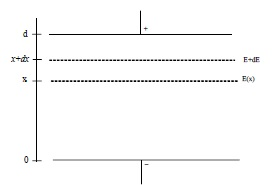
\includegraphics[width=\linewidth]{V_A1}}
	\caption{Схема расположения электродов в диоде}
	\label{mah}
	\vspace{-2cm}
\end{wrapfigure}

\par В случае цилиндрической симметрии решение уравнения записывается в виде:
\begin{equation}
I = \frac{8 \sqrt{2} \pi \varepsilon_0 l}{9} \sqrt{\frac{e}{m}} \frac{1}{r_a \beta^2} V^{3/2}
\end{equation}
\par где $\beta^2$ функция от $r_a/r_k$, которая может быть задана бесконечным рядом или графиком, $r_a,r_k$ - радиусы катода и анода в случае циллиндрического диода. То обстоятельство, что $I$ пропорционально $V^{3/2}$, уже обсуждалось. Линейный характер связи между $I$ и $\sqrt{e/m}$ очевиден из рассмотрения правой части (9). Численный коэффициент при $V^{3/2}$ выбран так, чтобы $r_a/r_k \to \infty$ при $\beta^2 \to 1$.

\section{Экспериментальная установка}
\begin{figure} [h]
	\centering
	\fbox{
		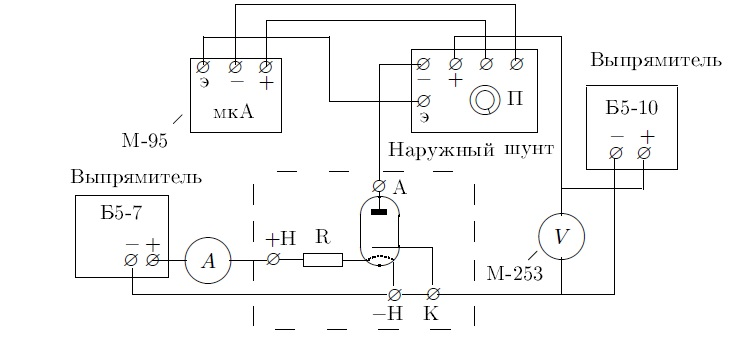
\includegraphics[width=\linewidth]{V_A2}}
	\caption{Схема экспериментальной установки}
	\label{mah}
\end{figure}
\par Исследования проводятся на диоде 2Ц2С с косвенным накалом. Радиус его катода $r_k$ = 0,9 мм, радиус анода $r_a$ = 9,5 мм, коэффициент $\beta ^2$ = 0,98. Полная высота анода и катода составляет около 20 мм, однако эмиссия электронов происходит только с центральной части катода, покрытой оксидным слоем. Высота этого слоя $I$ = 9 мм. Поскольку рабочая часть катода достаточно удалена от его торцов, электрическое поле в этой части с хорошей точностью можно считать радиальным.
Схема экспериментальной установки изображена на рис. 2. Для подогрева катода используется стабилизированный выпрямитель Б5-7, а в качестве анодного источника — выпрямитель Б5-10. В цепь накала включены амперметр $А$ и предохранительное сопротивление $R$. Анодное напряжение измеряется вольтметром (многопредельным гальванометром М-253), а анодный ток — миллиамперметром (микроамперметром М-95 с наружным шунтом). Наружный шунт позволяет изменять пределы измерений тока от 10 мкА до 10 мА.

\section{Ход работы}

\par 1. Подготовим приборы к работе.
\par 2. Регулятором выпрямителя цепи накала установим ток накала 1,3 А.
\par 3. Регулятором выпрямителя анодной цепи установим анодное напряжение $V_a$ = 0,5 В.
\par 4. Исследуем вольт-амперные характеристики диода в диапазоне от 0 до 50 В. В процессе измерений тока накала постоянен. В диапазоне от 0 до 6 В изменяем напряжение шагами по 0,5 В, в диапазоне от 6 до 10 В — шагами по 1 В, а в диапазоне от 10 до 50 В — шагами по 5 В.
\par 5. Повторим измерения при токах накала 1,4; 1,5 и 1,6 А. Данные занесем в таблицу 1.

\begin{table}[h!]
	\centering
	\caption{ Экспериментальные данные }

\begin{tabular}{|c|c|c|c|c|c|}
	\hline 
	& & $I_n$ = 1,3 A & $I_n$ = 1,4 A & $I_n$ = 1,5 A & $I_n$ = 1,6 A \\ 
	\hline 
	$U$, B & $U^{3/2}$, B$^{3/2}$ & $I$, мкA & $I$, мкA & $I$, мкA & $I$, мкA \\ 
	\hline 
	0,5 & 0,35 & 5,5 & 7,3 & 12,7 & 21,5 \\ 
	\hline 
	1 & 1 & 13,9 & 17,5 & 25,4 & 38,1 \\ 
	\hline 
	1,5 & 1,84 & 25,7 & 30,3 & 40,8 & 55,7 \\ 
	\hline 
	2 & 2,83 & 37,6 & 45,9 & 57,6 & 72,3 \\ 
	\hline 
	2,5 & 3,95 & 54,9 & 62,5 & 76,8 & 94,2 \\ 
	\hline 
	3 & 5,2 & 69,4 & 80 & 95 & 113,4 \\ 
	\hline 
	3,5 & 6,55 & 87,4 & 98,6 & 115 & 135 \\ 
	\hline 
	4 & 8 & 106,5 & 121 & 137,3 & 161,6 \\ 
	\hline 
	4,5 & 9,55 & 125,6 & 141,6 & 160,4 & 183,5 \\ 
	\hline 
	5 & 11,18 & 148,8 & 164,6 & 184,9 & 209,2 \\ 
	\hline 
	5,5 & 12,9 & 170,6 & 188,7 & 210,6 & 235,8 \\ 
	\hline 
	6 & 14,7 & 193,9 & 212,2 & 232,5 & 266,9 \\ 
	\hline 
	7 & 18,52 & 243,7 & 266,3 & 289,2 & 323,6 \\ 
	\hline 
	8 & 22,63 & 294,7 & 321,3 & 362,5 & 392,6 \\ 
	\hline 
	9 & 27 & 357,2 & 386,4 & 419,6 & 461,3 \\ 
	\hline 
	10 & 31,62 & 420,3 & 451,8 & 488,2 & 571,7 \\ 
	\hline 
	15 & 58,09 & 825 & 870,7 & 925,2 & 994,1 \\ 
	\hline 
	20 & 89,44 & 1308 & 1374,6 & 1440,5 & 1533,1 \\ 
	\hline 
	25 & 125 & 1874 & 1959,4 & 2045 & 2151,2 \\ 
	\hline 
	30 & 164,32 & 2504 & 2602,6 & 2697 & 2817,3 \\ 
	\hline 
	35 & 207,06 & 3181 & 3308,6 & 3419 & 3552,9 \\ 
	\hline 
	40 & 252,98 & 3906 & 4059,5 & 4193,5 & 4336,7 \\ 
	\hline 
	45 & 301,87 & 4692 & 4888,5 & 5016,5 & 5256 \\ 
	\hline 
	50 & 353,55 & 5588 & 5842 & 6005 & 6179 \\ 
	\hline 
\end{tabular} 
\end{table}

\section{Обработка результатов}

\par 1. По результатам эксперимента построим графики зависимости $I_a = f({V_a}^{3/2})$. Определим интервалы значений $V_a$, на которых графики имеют вид прямых линий. Найдем наклон прямолинейных участков характеристик и вычисленим $e/m$ электрона.
\begin{equation}
\frac{e}{m} = \frac{81 \cdot k^2 \cdot r_{\alpha}^2 \cdot \beta^4}{128 \cdot \pi^2 \cdot \varepsilon_0^2 \cdot l^2}
\end{equation}

\par Оценим погрешности эксперимента.
\begin{equation}
\Delta \big(\frac{e}{m}\big) = 2\Delta k \cdot 876 \cdot 10^{18}
\end{equation}

\par $\big(\frac{e}{m}\big)_1 = (2,1868 \pm 0,0011) \cdot 10^{11}$ Кл/кг
\par $\big(\frac{e}{m}\big)_2 = (2,3389 \pm 0,0007) \cdot 10^{11}$ Кл/кг
\par $\big(\frac{e}{m}\big)_3 = (2,4547 \pm 0,0007) \cdot 10^{11}$ Кл/кг
\par $\big(\frac{e}{m}\big)_4 = (2,5825 \pm 0,0005) \cdot 10^{11}$ Кл/кг

\begin{figure} 
	\centering
	\fbox{
		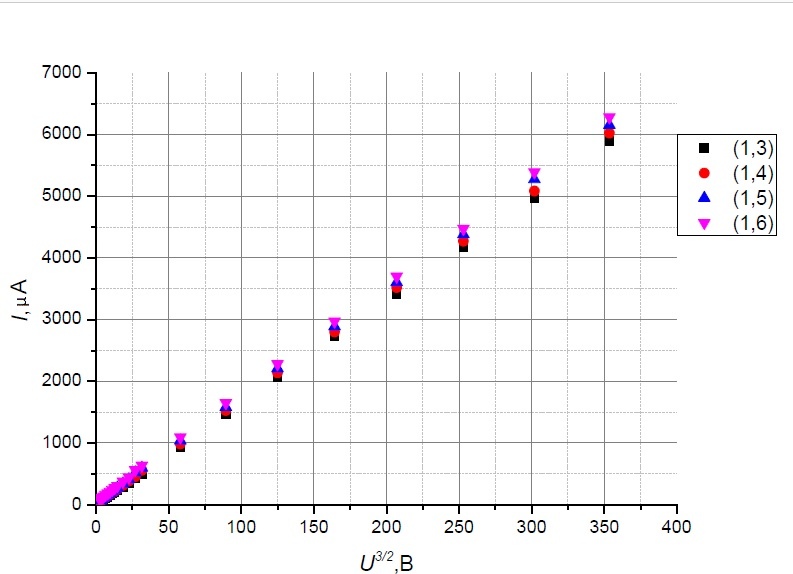
\includegraphics[width=\linewidth]{V_A_A5}}
	\caption{Вольт-амперная характеристика для всех токов накала}
	\label{mah}
\end{figure}

\begin{figure} 
	\centering
	\fbox{
		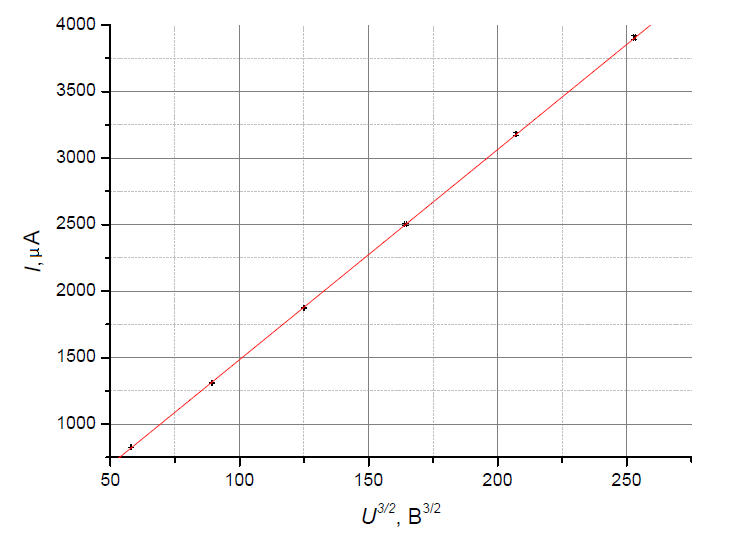
\includegraphics[width=\linewidth]{V_A_A1_1}}
	\caption{Вольт-амперная характеристика для тока накала $I_n = 1,3$ A, $k_1 = (15,80 \pm 0,06)$ $\mu A/U^{3/2}$}
	\label{mah}
\end{figure}

\begin{figure} 
	\centering
	\fbox{
		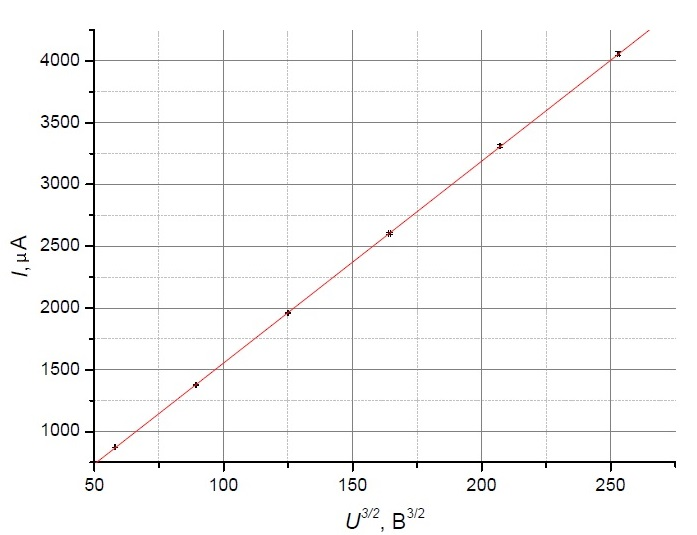
\includegraphics[width=\linewidth]{V_A_A2_1}}
	\caption{Вольт-амперная характеристика для тока накала $I_n = 1,4$ A, $k_2 = (16,34 \pm 0,04)$ $\mu A/U^{3/2}$}
	\label{mah}
\end{figure}

\begin{figure} 
	\centering
	\fbox{
		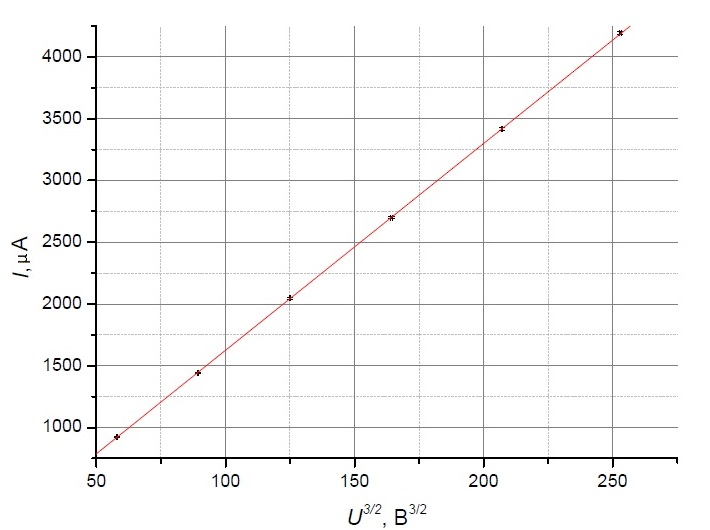
\includegraphics[width=\linewidth]{V_A_A3_1}}
	\caption{Вольт-амперная характеристика для тока накала $I_n = 1,5$ A, $k_3 = 16,74 \pm 0,04$}
	\label{mah}
\end{figure}

\begin{figure} 
	\centering
	\fbox{
		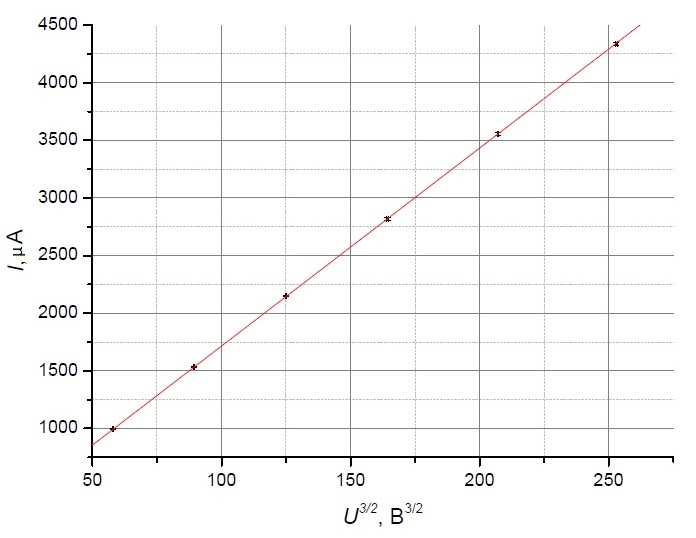
\includegraphics[width=\linewidth]{V_A_A4_1}}
	\caption{Вольт-амперная характеристика для тока накала $I_n = 1,6$ A, $k_4 = (17,17 \pm 0,03)$ $\mu A/U^{3/2}$}
	\label{mah}
\end{figure}

\par 2. В тех же координатах на других рисунках построим участоки вольт-амперной характеристики в диапазоне анодных напряжений от 0 до 10 В(рис.8 - 11). 

\begin{figure} 
	\centering
	\fbox{
		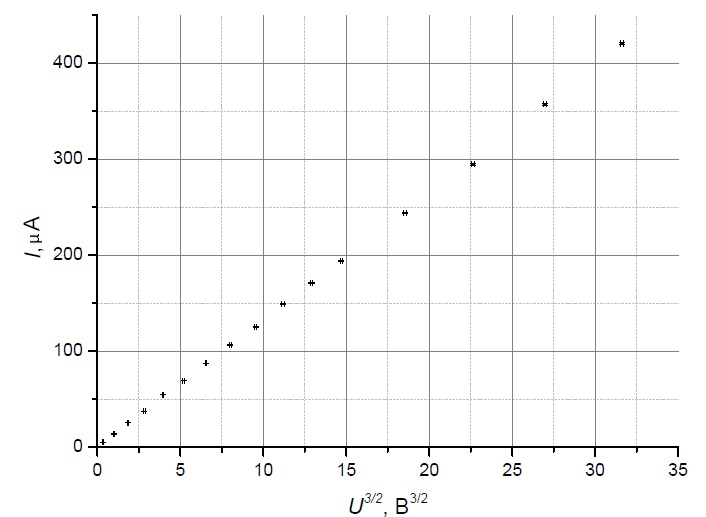
\includegraphics[width=\linewidth]{V_A_A1_2}}
	\caption{Вольт-амперная характеристика для тока накала $I_n = 1,3$ A}
	\label{mah}
\end{figure}

\begin{figure} 
	\centering
	\fbox{
		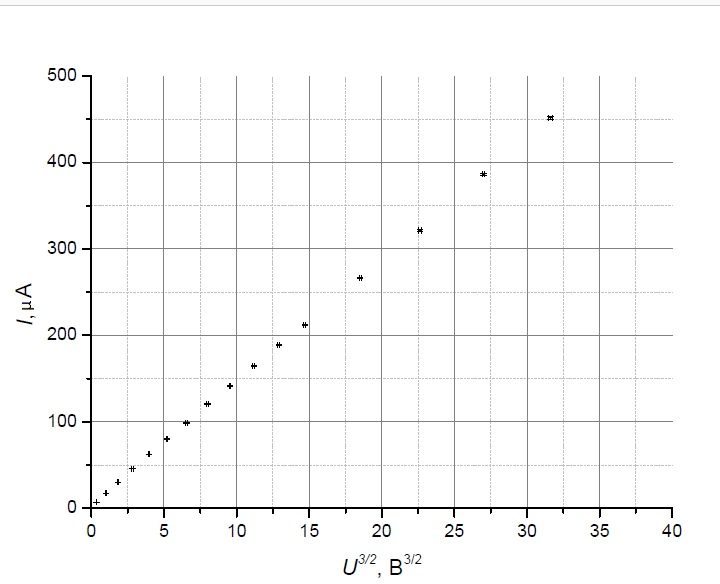
\includegraphics[width=\linewidth]{V_A_A2_2}}
	\caption{Вольт-амперная характеристика для тока накала $I_n = 1,4$ A}
	\label{mah}
\end{figure}

\begin{figure} 
	\centering
	\fbox{
		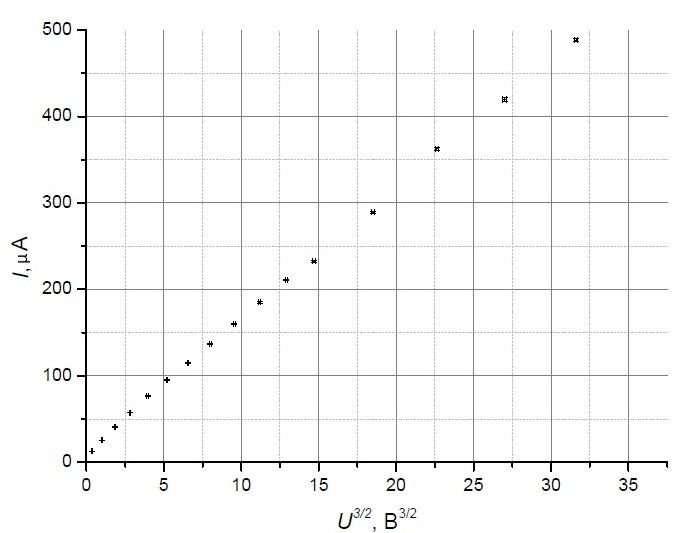
\includegraphics[width=\linewidth]{V_A_A3_2}}
	\caption{Вольт-амперная характеристика для тока накала $I_n = 1,5$ A}
	\label{mah}
\end{figure}

\begin{figure} 
	\centering
	\fbox{
		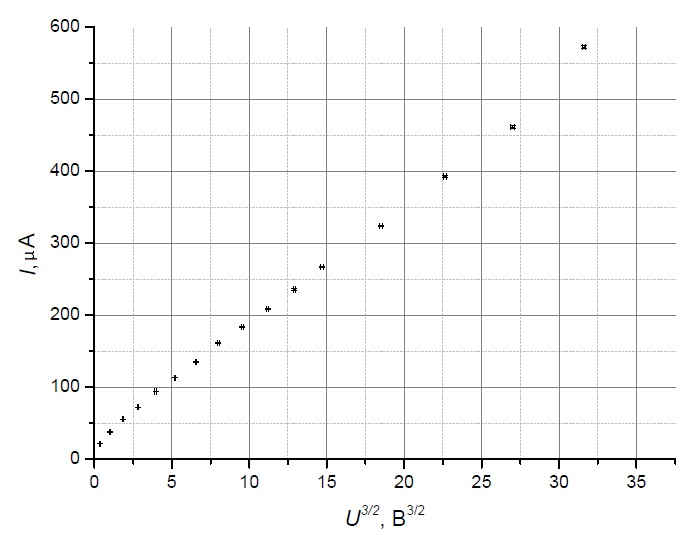
\includegraphics[width=\linewidth]{V_A_A4_2}}
	\caption{Вольт-амперная характеристика для тока накала $I_n = 1,6$ A}
	\label{mah}
\end{figure}

\section{Обсуждение результатов и выводы}
\par В ходе данной работы была получена вольт-амперная характеристика вакуумного диода. Были получены участки, на которых выполняется закон "трех вторых" для разных токов накала. По наклону прямолинейных участков было определено отношение заряда электрона к его массе. Наиболее достоверный результат $\big(\frac{e}{m}\big)_1 = (2,1868 \pm 0,0011) \cdot 10^{11}$ Кл/кг, табличное  $\frac{e}{m} = 1,7579 \cdot 10^{11}$ Кл/кг. Результаты не сошлись.
\end{document}